\chapter{Dynamics in Non-Inertial Reference Frames}
\label{ch:noninertial}
\begin{chapterintro}
\textbf{You will learn to:} distinguish inertial from non-inertial frames; compute the fictitious forces of transport and Coriolis; formulate Newton's second law in a moving frame; analyse apparent weight and the shape of rotating fluids; and calculate the eastward deflection of falling bodies and the precession of the Foucault pendulum.
\end{chapterintro}

\section{Inertial vs Non-Inertial Frames}

Newton's laws of motion are valid only in \textbf{inertial (Galilean) reference frames}---frames that are either at rest or moving at constant velocity with respect to the distant stars.

When we observe motion from an \textbf{accelerating or rotating reference frame} $\mathcal{R}'(O', x', y', z')$ relative to an inertial frame $\mathcal{R}(O, x, y, z)$, the frame itself experiences acceleration. To apply Newton's second law in $\mathcal{R}'$, we must introduce \textbf{fictitious (inertial) forces}. These forces do not arise from physical interactions (no physical agent pulls on the body), but are purely consequences of the acceleration of the observer's frame.

\begin{figure}[htbp]
\centering
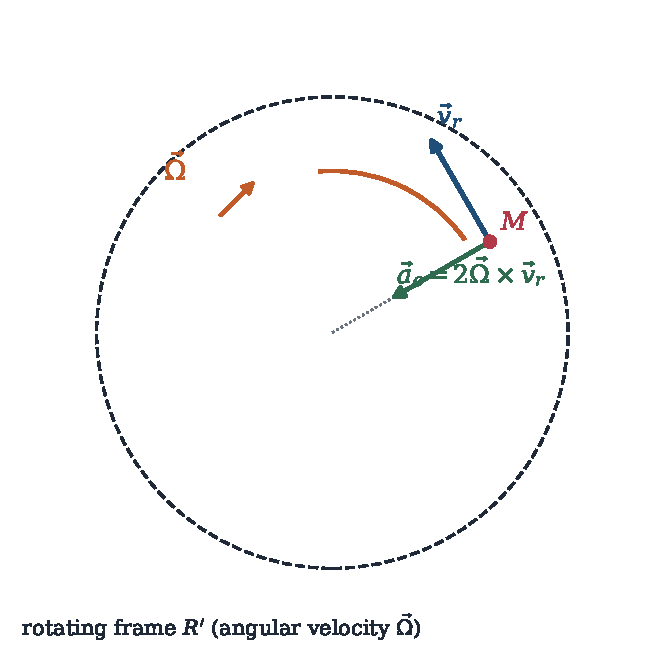
\includegraphics[width=0.72\textwidth]{figures/10_rotating_frame.pdf}
\caption{A particle $M$ observed from both a fixed inertial frame $\mathcal{R}(O,\ihat,\jhat,\khat)$ and a rotating frame $\mathcal{R}'(O',\ur,\ut,\khat)$ with angular velocity $\vec{\Omega}$.}
\label{fig:rotating_frame}
\end{figure}

\section{Composition of Accelerations and Fictitious Forces}

Recall from kinematics that the absolute acceleration $\vec{a}_a$ of a particle of mass $m$ is related to its relative acceleration $\vec{a}_r$ in $\mathcal{R}'$ by:
\[
\vec{a}_a = \vec{a}_r + \vec{a}_e + \vec{a}_c,
\]
where:
\begin{itemize}[leftmargin=1.4em,itemsep=3pt]
  \item $\vec{a}_r = \left(\frac{\dd^2\vec{r}'}{\dd t^2}\right)_{\mathcal{R}'}$ is the \textbf{relative acceleration} observed in $\mathcal{R}'$;
  \item $\vec{a}_e = \vec{a}(O') + \left(\frac{\dd\vec{\Omega}}{\dd t}\right)\times\vec{r}' + \vec{\Omega}\times(\vec{\Omega}\times\vec{r}')$ is the \textbf{acceleration of transport} (acceleration of the point in $\mathcal{R}'$ coincident with $M$);
  \item $\vec{a}_c = 2\vec{\Omega}\times\vec{v}_r$ is the \textbf{Coriolis acceleration}.
\end{itemize}

Multiplying by mass $m$ and using Newton's second law in the inertial frame, $m\vec{a}_a = \sum\vec{F}_{\text{real}}$, we obtain the \textbf{Fundamental Equation of Relative Dynamics}:
\[
\boxed{m\vec{a}_r = \sum\vec{F}_{\text{real}} + \vec{F}_{ie} + \vec{F}_{ic}}
\]
where the two inertial forces are:
\begin{align}
\vec{F}_{ie} &= -m\vec{a}_e \quad \text{(\textbf{Inertial force of transport / Centrifugal force})}, \\
\vec{F}_{ic} &= -m\vec{a}_c = -2m\,\vec{\Omega}\times\vec{v}_r \quad \text{(\textbf{Coriolis force})}.
\end{align}

\begin{keyidea}[Characteristics of Fictitious Forces]
\begin{itemize}[leftmargin=1.4em,itemsep=2pt]
  \item $\vec{F}_{ie}$ exists whenever the frame translates with acceleration ($\vec{a}(O')\ne\vzero$) or rotates. In a purely rotating frame ($\vec{\Omega} = \text{const}$, $O'=O$), $\vec{F}_{ie} = -m\vec{\Omega}\times(\vec{\Omega}\times\vec{r}') = m\Omega^2\vec{r}_\perp$ is directed \emph{radially outward} from the axis of rotation: the \textbf{centrifugal force}.
  \item $\vec{F}_{ic}$ acts \textbf{only when the particle is moving} in the relative frame ($\vec{v}_r\ne\vzero$). It is always perpendicular to the relative velocity ($\vec{F}_{ic}\cdot\vec{v}_r = 0$), meaning \textbf{the Coriolis force does no mechanical work} in the relative frame!
\end{itemize}
\end{keyidea}

\begin{method}[Solving Dynamics in a Non-Inertial Frame]
\begin{enumerate}[leftmargin=1.5em,itemsep=2pt]
  \item Identify the relative frame $\mathcal{R}'$ and its acceleration $\vec{a}(O')$ and angular velocity $\vec{\Omega}(t)$.
  \item Draw the free-body diagram of the particle including all \textbf{real forces} ($\vec{P}, \vec{N}, \vec{T}, \vec{f}$, etc.).
  \item Add the \textbf{fictitious forces}: $\vec{F}_{ie} = -m\vec{a}_e$ and $\vec{F}_{ic} = -2m\vec{\Omega}\times\vec{v}_r$.
  \item Apply $m\vec{a}_r = \sum\vec{F}_{\text{real}} + \vec{F}_{ie} + \vec{F}_{ic}$ along chosen coordinate axes in $\mathcal{R}'$.
\end{enumerate}
\end{method}

\section{Worked Examples}

\begin{worked}[Incline inside an accelerating truck]
A block of mass $m=2.0\ \mathrm{kg}$ sits on a smooth ramp of angle $\alpha=30^\circ$ fixed inside a truck. The truck accelerates horizontally with acceleration $a_0$. Find the acceleration $a_0$ such that the block remains at rest relative to the ramp.
\end{worked}

\begin{solution}{10.1}
In the frame of the truck $\mathcal{R}'$ (translating horizontally with $\vec{a}_0 = a_0\ihat$):
\begin{itemize}[leftmargin=1.4em,itemsep=2pt]
  \item Real forces: weight $\vec{P} = -mg\jhat$, normal force $\vec{N}$ perpendicular to the ramp ($N\sin\alpha\ihat + N\cos\alpha\jhat$).
  \item Fictitious force: $\vec{F}_{ie} = -m\vec{a}_0 = -m a_0\ihat$. Since $\vec{\Omega}=\vzero$, $\vec{F}_{ic}=\vzero$.
\end{itemize}
Relative equilibrium requires $\vec{a}_r = \vzero$, hence:
\[
\vec{P} + \vec{N} + \vec{F}_{ie} = \vzero.
\]
Projecting along the horizontal and vertical axes:
\begin{align*}
\text{Horizontal:}\quad & N\sin\alpha - m a_0 = 0 \implies N\sin\alpha = m a_0, \\
\text{Vertical:}\quad & N\cos\alpha - mg = 0 \implies N\cos\alpha = mg.
\end{align*}
Dividing the two equations eliminates $N$:
\[
\tan\alpha = \frac{a_0}{g} \implies \boxed{a_0 = g\tan\alpha.}
\]
For $\alpha=30^\circ$, $a_0 = 9.81\times\tan 30^\circ = 9.81\times 0.577 = 5.66\ \mathrm{m\,s^{-2}}$.
\end{solution}

\begin{worked}[Bead sliding on a rotating smooth rod]
A thin smooth horizontal rod rotates about a vertical axis through one end $O$ at constant angular velocity $\omega$. A bead of mass $m$ slides along the rod with distance $r(t)$ from $O$. Find the equation of motion for $r(t)$ and the horizontal reaction force exerted by the rod.
\end{worked}

\begin{solution}{10.2}
In the rotating frame $\mathcal{R}'$ attached to the rod with unit vector $\ur$ along the rod and $\ut$ perpendicular:
\begin{itemize}[leftmargin=1.4em,itemsep=2pt]
  \item The relative position is $\vec{r}' = r\ur$, relative velocity $\vec{v}_r = \dot{r}\ur$, relative acceleration $\vec{a}_r = \ddot{r}\ur$.
  \item Real forces: weight $\vec{P} = -mg\khat$, normal reaction $\vec{N} = N_\theta\ut + N_z\khat$ (since the rod is smooth, there is no component along $\ur$).
  \item Centrifugal force: $\vec{F}_{\text{cf}} = -m\vec{\Omega}\times(\vec{\Omega}\times\vec{r}') = m\omega^2 r\ur$.
  \item Coriolis force: $\vec{F}_{\text{Cor}} = -2m\vec{\Omega}\times\vec{v}_r = -2m(\omega\khat)\times(\dot{r}\ur) = -2m\omega\dot{r}\ut$.
\end{itemize}
Applying $m\vec{a}_r = \vec{P} + \vec{N} + \vec{F}_{\text{cf}} + \vec{F}_{\text{Cor}}$:
\begin{align*}
\ur:\quad & m\ddot{r} = m\omega^2 r \implies \boxed{\ddot{r} - \omega^2 r = 0,} \\
\ut:\quad & 0 = N_\theta - 2m\omega\dot{r} \implies \boxed{N_\theta = 2m\omega\dot{r},} \\
\khat:\quad & 0 = N_z - mg \implies N_z = mg.
\end{align*}
The radial equation $\ddot{r} - \omega^2 r = 0$ has solution $r(t) = A\cosh(\omega t) + B\sinh(\omega t)$. The bead accelerates exponentially outward! The rod must push horizontally with $N_\theta = 2m\omega\dot{r}$ to counteract the Coriolis force.
\end{solution}

\section{Exercises and Step-by-Step Solutions}

\begin{exercise}{\warm\ Scale in an accelerating elevator}
A student of mass $m=70.0\ \mathrm{kg}$ stands on a spring scale inside an elevator. What does the scale read (in newtons and equivalent apparent mass in $\mathrm{kg}$) when:
(a) the elevator accelerates upward at $a=2.00\ \mathrm{m\,s^{-2}}$;
(b) the elevator moves upward at constant speed $v=4.00\ \mathrm{m\,s^{-1}}$;
(c) the elevator accelerates downward at $a=2.00\ \mathrm{m\,s^{-2}}$;
(d) the elevator cable snaps and it falls freely?
\end{exercise}

\begin{tabletworkspace}[5.5cm]
\end{tabletworkspace}

\begin{solution}{10.1}
In the reference frame of the elevator $\mathcal{R}'$, the elevator has vertical acceleration $\vec{a} = a\jhat$ (with $\jhat$ upward).
The forces acting on the student in $\mathcal{R}'$ are:
\begin{itemize}[leftmargin=1.4em,itemsep=2pt]
  \item Real weight: $\vec{P} = -mg\jhat$;
  \item Normal reaction from the scale: $\vec{N} = N\jhat$ (the scale reads $N$);
  \item Fictitious inertial force: $\vec{F}_{ie} = -m\vec{a}_e = -m a\jhat$.
\end{itemize}
Since the student is at rest in the elevator ($\vec{a}_r = \vzero$):
\[
\vec{N} + \vec{P} + \vec{F}_{ie} = \vzero \implies N - mg - ma = 0 \implies N = m(g + a).
\]
(a) Accelerating upward ($a = +2.00\ \mathrm{m\,s^{-2}}$):
\[
N = 70.0(9.81 + 2.00) = 70.0(11.81) = 826.7\ \mathrm{N}.
\]
Apparent mass reading: $m_{\text{app}} = N/g = 826.7/9.81 = 84.3\ \mathrm{kg}$.

(b) Constant speed ($a = 0$):
\[
N = mg = 70.0\times 9.81 = 686.7\ \mathrm{N} \implies m_{\text{app}} = 70.0\ \mathrm{kg}.
\]

(c) Accelerating downward ($a = -2.00\ \mathrm{m\,s^{-2}}$):
\[
N = m(g - 2.00) = 70.0(9.81 - 2.00) = 70.0(7.81) = 546.7\ \mathrm{N} \implies m_{\text{app}} = 55.7\ \mathrm{kg}.
\]

(d) Free fall ($a = -g$):
\[
N = m(g - g) = 0\ \mathrm{N} \implies m_{\text{app}} = 0\ \mathrm{kg}\quad \text{(weightlessness)}.
\]
\end{solution}

\begin{exercise}{\warm\ Direction and magnitude of the Coriolis force}
A bullet of mass $m=20.0\ \mathrm{g}$ is fired horizontally due north at speed $v=800\ \mathrm{m\,s^{-1}}$ at a location in the Northern hemisphere with latitude $\lambda=45.0^\circ$.
(a) Determine the direction of the Coriolis force $\vec{F}_{\text{Cor}} = -2m\vec{\Omega}\times\vec{v}_r$.
(b) Calculate the magnitude of $\vec{F}_{\text{Cor}}$, given Earth's angular speed $\Omega \approx 7.292\times 10^{-5}\ \mathrm{rad\,s^{-1}}$.
(c) Compare this force with the bullet's weight $mg$.
\end{exercise}

\begin{tabletworkspace}[5.5cm]
\end{tabletworkspace}

\begin{solution}{10.2}
Set up a local coordinate frame with $\ihat$ pointing East, $\jhat$ pointing North, and $\khat$ pointing vertically upward (Zenith).
Earth's angular velocity vector $\vec{\Omega}$ points parallel to Earth's polar axis (North):
\[
\vec{\Omega} = \Omega\cos\lambda\jhat + \Omega\sin\lambda\khat.
\]
(a) The bullet flies horizontally due North: $\vec{v}_r = v\jhat$.
The cross product is:
\[
\vec{\Omega}\times\vec{v}_r = (\Omega\cos\lambda\jhat + \Omega\sin\lambda\khat)\times(v\jhat) = -\Omega v\sin\lambda\,\ihat.
\]
Therefore, the Coriolis force is:
\[
\vec{F}_{\text{Cor}} = -2m(\vec{\Omega}\times\vec{v}_r) = +2m\Omega v\sin\lambda\,\ihat.
\]
Since $\ihat$ is East, the Coriolis force is directed \textbf{due East} (deflecting the trajectory to the right).

(b) Magnitude:
\[
F_{\text{Cor}} = 2m\Omega v\sin\lambda = 2(0.0200)(7.292\times 10^{-5})(800)\sin 45^\circ = 2(0.0200)(7.292\times 10^{-5})(800)(0.7071) \approx 1.65\times 10^{-3}\ \mathrm{N}.
\]

(c) The weight is $P = mg = 0.0200\times 9.81 = 0.1962\ \mathrm{N}$.
The ratio is:
\[
\frac{F_{\text{Cor}}}{mg} = \frac{1.65\times 10^{-3}}{0.1962} \approx 8.4\times 10^{-3} \approx 0.84\%.
\]
Although small, over long trajectories (such as artillery shells or storm systems), this deflection is significant.
\end{solution}

\begin{exercise}{\core\ Plumb line deflection and apparent gravity}
Because the Earth rotates with angular speed $\Omega$ about its North-South axis, a plumb line does not point exactly toward the Earth's geometric center $O$.
(a) Show that the effective gravity $\vec{g}_{\text{eff}}$ at latitude $\lambda$ is given by $\vec{g}_{\text{eff}} = \vec{g}_0 + \Omega^2 R_E\cos\lambda\,\vec{u}_\perp$, where $\vec{g}_0 = -(GM_E/R_E^2)\vec{u}_r$ and $\vec{u}_\perp$ is directed perpendicular to the rotation axis outward.
(b) Find an expression for the deflection angle $\theta$ between the true vertical and the plumb line, assuming $\Omega^2 R_E \ll g_0$.
(c) Calculate the maximum deflection angle $\theta_{\max}$ and the latitude at which it occurs (take $R_E = 6.37\times 10^6\ \mathrm{m}$).
\end{exercise}

\begin{tabletworkspace}[6.0cm]
\end{tabletworkspace}

\begin{solution}{10.3}
(a) A plumb bob of mass $m$ hanging at rest relative to Earth ($\vec{v}_r = \vzero$) is in equilibrium under its true gravitational attraction $\vec{F}_g = m\vec{g}_0$, the string tension $\vec{T}$, and the centrifugal force $\vec{F}_{\text{cf}}$:
\[
\vec{T} + m\vec{g}_0 + \vec{F}_{\text{cf}} = \vzero.
\]
The apparent weight is defined as $\vec{P}_{\text{app}} = -\vec{T} = m\vec{g}_{\text{eff}}$. Thus:
\[
m\vec{g}_{\text{eff}} = m\vec{g}_0 + \vec{F}_{\text{cf}}.
\]
The distance from the bob to the rotation axis is $r_\perp = R_E\cos\lambda$. The centrifugal force is:
\[
\vec{F}_{\text{cf}} = m\Omega^2 r_\perp\vec{u}_\perp = m\Omega^2 R_E\cos\lambda\,\vec{u}_\perp.
\]
Dividing by $m$ yields:
\[
\vec{g}_{\text{eff}} = \vec{g}_0 + \Omega^2 R_E\cos\lambda\,\vec{u}_\perp.
\]

(b) Resolve $\vec{u}_\perp$ into local radial ($-\ur$, downward) and tangential ($\ut$, Southward) components:
\[
\vec{u}_\perp = \cos\lambda\,\ur - \sin\lambda\,\ut.
\]
Thus:
\begin{align*}
g_{\text{eff}, r} &= -g_0 + \Omega^2 R_E\cos^2\lambda \approx -g_0, \\
g_{\text{eff}, \theta} &= -\Omega^2 R_E\cos\lambda\sin\lambda = -\frac{1}{2}\Omega^2 R_E\sin(2\lambda).
\end{align*}
The deflection angle $\theta$ is small, so:
\[
\tan\theta \approx \theta \approx \frac{\abs{g_{\text{eff}, \theta}}}{\abs{g_{\text{eff}, r}}} \approx \frac{\Omega^2 R_E\sin(2\lambda)}{2g_0}.
\]

(c) The factor $\sin(2\lambda)$ reaches its maximum value of $1$ when $2\lambda = 90^\circ \implies \lambda = 45^\circ$.
At $\lambda = 45^\circ$:
\[
\theta_{\max} = \frac{\Omega^2 R_E}{2g_0} = \frac{(7.292\times 10^{-5})^2\times(6.37\times 10^6)}{2\times 9.81} = \frac{3.387\times 10^{-2}}{19.62} \approx 1.73\times 10^{-3}\ \mathrm{rad} \approx 0.099^\circ \approx 5.9'.
\]
The plumb line is deflected toward the equator by about $6$ arcminutes at $45^\circ$ latitude!
\end{solution}

\begin{exercise}{\core\ Liquid surface in an accelerating container}
A rectangular beaker of water is placed on a cart that accelerates horizontally with constant acceleration $a_0$ along the $+x$ direction.
(a) In the non-inertial frame of the beaker, determine the effective gravity $\vec{g}_{\text{eff}} = \vec{g} - \vec{a}_0$.
(b) Explain why the free surface of the liquid must be perpendicular to $\vec{g}_{\text{eff}}$.
(c) Deduce the angle of inclination $\theta$ of the liquid surface relative to the horizontal.
\end{exercise}

\begin{tabletworkspace}[5.5cm]
\end{tabletworkspace}

\begin{solution}{10.4}
(a) In the frame of the container $\mathcal{R}'$, each element of liquid experiences real gravity $\vec{g} = -g\jhat$ and the inertial force per unit mass $\vec{f}_{ie} = -\vec{a}_0 = -a_0\ihat$.
The effective gravitational acceleration in $\mathcal{R}'$ is:
\[
\vec{g}_{\text{eff}} = \vec{g} - \vec{a}_0 = -a_0\ihat - g\jhat.
\]

(b) At hydrostatic equilibrium in the relative frame, the pressure gradient satisfies $\vec{\nabla} p = \rho\vec{g}_{\text{eff}}$.
Along the free surface, the pressure is constant ($p = p_{\text{atm}}$), so $\dd p = \vec{\nabla} p\cdot\dd\vec{r} = 0$.
Therefore:
\[
\rho\vec{g}_{\text{eff}}\cdot\dd\vec{r} = 0 \implies \vec{g}_{\text{eff}}\perp\dd\vec{r}.
\]
The free surface must everywhere be orthogonal to the effective gravity vector $\vec{g}_{\text{eff}}$.

(c) Let the surface profile be $y(x)$. A tangent vector to the surface is $\dd\vec{r} = \dd x\ihat + \dd y\jhat$. The condition $\vec{g}_{\text{eff}}\cdot\dd\vec{r} = 0$ gives:
\[
(-a_0)\dd x + (-g)\dd y = 0 \implies \frac{\dd y}{\dd x} = -\frac{a_0}{g}.
\]
The surface is a flat plane tilted at an angle $\theta$ relative to the horizontal, with:
\[
\boxed{\tan\theta = \frac{a_0}{g}.}
\]
The liquid rises at the rear of the container and drops at the front.
\end{solution}

\begin{exercise}{\core\ Parabolic mirror: fluid in a rotating cylinder}
A cylindrical bucket containing liquid of density $\rho$ rotates about its central vertical axis at constant angular velocity $\omega$.
(a) Set up cylindrical coordinates $(r, \theta, z)$ in the rotating frame and find the effective force per unit volume on a fluid element.
(b) Integrate the hydrostatic equation $\vec{\nabla} p = \rho\vec{g}_{\text{eff}}$ to find the pressure distribution $p(r, z)$.
(c) Show that the free surface of the liquid forms a paraboloid of revolution, $z(r) = z_0 + \frac{\omega^2 r^2}{2g}$.
\end{exercise}

\begin{tabletworkspace}[6.0cm]
\end{tabletworkspace}

\begin{solution}{10.5}
(a) In the rotating frame $\mathcal{R}'$, the fluid is at rest. The forces per unit mass are gravity $\vec{g} = -g\khat$ and the centrifugal acceleration $\vec{a}_{\text{cf}} = \omega^2 r\ur$.
The effective field is:
\[
\vec{g}_{\text{eff}} = \omega^2 r\ur - g\khat.
\]
(Coriolis force is zero because $\vec{v}_r = \vzero$).

(b) Hydrostatic equilibrium in $\mathcal{R}'$:
\[
\vec{\nabla} p = \rho\vec{g}_{\text{eff}} \implies \frac{\partial p}{\partial r}\ur + \frac{1}{r}\frac{\partial p}{\partial \theta}\ut + \frac{\partial p}{\partial z}\khat = \rho\omega^2 r\ur - \rho g\khat.
\]
Matching components:
\[
\frac{\partial p}{\partial r} = \rho\omega^2 r,\qquad \frac{\partial p}{\partial \theta} = 0,\qquad \frac{\partial p}{\partial z} = -\rho g.
\]
Integrating:
\[
p(r, z) = p_0 + \frac{1}{2}\rho\omega^2 r^2 - \rho gz,
\]
where $p_0 = p(0, 0)$.

(c) Along the free surface, the pressure is atmospheric pressure $p_{\text{atm}}$. Setting $p(r, z) = p_{\text{atm}}$:
\[
p_{\text{atm}} = p_0 + \frac{1}{2}\rho\omega^2 r^2 - \rho gz \implies \rho gz = (p_0 - p_{\text{atm}}) + \frac{1}{2}\rho\omega^2 r^2.
\]
Defining $z_0 = z(0) = \frac{p_0 - p_{\text{atm}}}{\rho g}$:
\[
\boxed{z(r) = z_0 + \frac{\omega^2 r^2}{2g}.}
\]
This is a paraboloid of revolution! This principle is used in liquid-mirror astronomical telescopes (using molten gallium or mercury).
\end{solution}

\begin{exercise}{\core\ Mass on a rotating turntable with friction}
A small puck of mass $m=0.30\ \mathrm{kg}$ sits on a horizontal rotating turntable at a distance $r=0.25\ \mathrm{m}$ from the axis of rotation. The coefficient of static friction between puck and turntable is $\mu_s=0.40$.
(a) In the turntable frame, write the force balance condition for the puck to remain stationary.
(b) Calculate the maximum angular velocity $\omega_{\max}$ (in $\mathrm{rad\,s^{-1}}$ and in $\mathrm{rpm}$) before the puck slips.
(c) If the turntable rotates at $\omega = 5.0\ \mathrm{rad\,s^{-1}}$ and the puck is pushed radially inward with speed $v_r = 0.50\ \mathrm{m\,s^{-1}}$, compute the Coriolis force acting on it.
\end{exercise}

\begin{tabletworkspace}[5.5cm]
\end{tabletworkspace}

\begin{solution}{10.6}
(a) In the rotating frame of the turntable:
\begin{itemize}[leftmargin=1.4em,itemsep=2pt]
  \item Vertical: normal force $\vec{N} = N\khat$ balances weight $\vec{P} = -mg\khat \implies N = mg$.
  \item Horizontal: the centrifugal force $\vec{F}_{\text{cf}} = m\omega^2 r\ur$ pulls radially outward. To remain stationary ($\vec{v}_r = \vzero, \vec{a}_r = \vzero$), static friction $\vec{f}_s$ must point radially inward: $\vec{f}_s = -m\omega^2 r\ur$.
\end{itemize}
The condition for no slip is $f_s \le \mu_s N$:
\[
m\omega^2 r \le \mu_s mg \implies \omega^2 r \le \mu_s g.
\]

(b) Maximum angular velocity:
\[
\omega_{\max} = \sqrt{\frac{\mu_s g}{r}} = \sqrt{\frac{0.40\times 9.81}{0.25}} = \sqrt{15.696} \approx 3.96\ \mathrm{rad\,s^{-1}}.
\]
In revolutions per minute:
\[
N_{\text{rpm}} = \frac{\omega_{\max}\times 60}{2\pi} = \frac{3.96\times 60}{2\pi} \approx 37.8\ \mathrm{rpm}.
\]

(c) If the puck has relative velocity $\vec{v}_r = -v_r\ur$ (radially inward):
Earth's rotation vector is $\vec{\Omega} = \omega\khat$. The Coriolis force is:
\[
\vec{F}_{\text{Cor}} = -2m\vec{\Omega}\times\vec{v}_r = -2m(\omega\khat)\times(-v_r\ur) = +2m\omega v_r(\khat\times\ur) = 2m\omega v_r\ut.
\]
The Coriolis force pushes in the direction of rotation ($\ut$, forward tangential).
Magnitude:
\[
F_{\text{Cor}} = 2(0.30)(5.0)(0.50) = 1.50\ \mathrm{N}.
\]
\end{solution}

\begin{exercise}{\mastery\ Eastward deflection of a falling body}
A stone is dropped from rest from the top of a tower of height $h=100\ \mathrm{m}$ at latitude $\lambda=45^\circ$ in the Northern hemisphere.
(a) Using the coordinate system ($\ihat$ East, $\jhat$ North, $\khat$ Zenith), write the equations of motion for the stone in the Earth-bound frame including gravity and the Coriolis force (neglect the centrifugal term $\Omega^2 R_E$ and air resistance).
(b) By successive approximations (first-order in $\Omega$), show that the stone is deflected toward the East by an amount:
\[
d_E = \frac{1}{3}\Omega\cos\lambda\sqrt{\frac{8h^3}{g}}.
\]
(c) Calculate the numerical value of $d_E$.
\end{exercise}

\begin{tabletworkspace}[6.5cm]
\end{tabletworkspace}

\begin{solution}{10.7}
(a) In the local frame, $\vec{\Omega} = \Omega\cos\lambda\jhat + \Omega\sin\lambda\khat$.
The velocity is $\vec{v}_r = \dot{x}\ihat + \dot{y}\jhat + \dot{z}\khat$.
The Coriolis acceleration is:
\begin{align*}
\vec{a}_{\text{Cor}} &= -2\vec{\Omega}\times\vec{v}_r = -2\begin{vmatrix} \ihat & \jhat & \khat \\ 0 & \Omega\cos\lambda & \Omega\sin\lambda \\ \dot{x} & \dot{y} & \dot{z} \end{vmatrix} \\
&= -2\left[ (\dot{z}\Omega\cos\lambda - \dot{y}\Omega\sin\lambda)\ihat + (\dot{x}\Omega\sin\lambda)\jhat - (\dot{x}\Omega\cos\lambda)\khat \right].
\end{align*}
Newton's second law $m\vec{a}_r = m\vec{g} + \vec{F}_{\text{Cor}}$ yields the three scalar differential equations:
\begin{align*}
\ddot{x} &= 2\Omega(\dot{y}\sin\lambda - \dot{z}\cos\lambda), \\
\ddot{y} &= -2\Omega\dot{x}\sin\lambda, \\
\ddot{z} &= -g + 2\Omega\dot{x}\cos\lambda.
\end{align*}

(b) At zeroth order in $\Omega$ (unperturbed vertical fall with $x(0)=y(0)=0, z(0)=h$ and $\vec{v}(0)=\vzero$):
\[
\dot{x}^{(0)} = 0,\quad \dot{y}^{(0)} = 0,\quad \ddot{z}^{(0)} = -g \implies \dot{z}^{(0)}(t) = -gt,\quad z^{(0)}(t) = h - \frac{1}{2}gt^2.
\]
The fall time to ground level ($z=0$) is $t_f = \sqrt{2h/g}$.

Now substitute the zeroth-order solution into the $\ddot{x}$ equation to find the first-order correction:
\[
\ddot{x}^{(1)} = 2\Omega(0 - (-gt)\cos\lambda) = 2\Omega gt\cos\lambda.
\]
Integrating twice with initial conditions $x(0)=0, \dot{x}(0)=0$:
\begin{align*}
\dot{x}(t) &= \Omega gt^2\cos\lambda, \\
x(t) &= \frac{1}{3}\Omega gt^3\cos\lambda.
\end{align*}
Since $x$ is along the East axis, the deflection is strictly \textbf{Eastward}!
Evaluating at $t = t_f = \sqrt{2h/g}$:
\[
d_E = x(t_f) = \frac{1}{3}\Omega g \left(\frac{2h}{g}\right)^{3/2}\cos\lambda = \boxed{\frac{1}{3}\Omega\cos\lambda\sqrt{\frac{8h^3}{g}}.}
\]

(c) Numerical calculation with $h=100\ \mathrm{m}, g=9.81\ \mathrm{m\,s^{-2}}, \Omega=7.292\times 10^{-5}\ \mathrm{rad\,s^{-1}}, \lambda=45^\circ$:
\[
t_f = \sqrt{\frac{2\times 100}{9.81}} = \sqrt{20.387} \approx 4.515\ \mathrm{s}.
\]
\[
d_E = \frac{1}{3}(7.292\times 10^{-5})(9.81)(4.515)^3\cos 45^\circ \approx 0.0155\ \mathrm{m} = \mathbf{1.55\ \mathrm{cm}}.
\]
The stone lands $1.55\ \mathrm{cm}$ East of the point directly below its release point.
\end{solution}

\begin{exercise}{\mastery\ Bead on a rotating vertical hoop}
A smooth circular wire hoop of radius $R$ is placed in a vertical plane and rotates about its vertical diameter with constant angular speed $\omega$. A bead of mass $m$ slides without friction on the hoop. The position of the bead is specified by the angle $\theta$ from the lowest point.
(a) In the rotating frame of the hoop, identify all real and fictitious forces acting on the bead.
(b) Project the equation of motion along the tangent to the hoop to show:
\[
R\ddot{\theta} = \left(\omega^2 R\cos\theta - g\right)\sin\theta.
\]
(c) Find all equilibrium angles $\theta_e$ and determine their stability as a function of the rotation speed $\omega$, identifying the critical threshold $\omega_c = \sqrt{g/R}$.
\end{exercise}

\begin{tabletworkspace}[6.5cm]
\end{tabletworkspace}

\begin{solution}{10.8}
(a) In the frame $\mathcal{R}'$ rotating with $\vec{\Omega} = \omega\khat$:
\begin{itemize}[leftmargin=1.4em,itemsep=2pt]
  \item Real forces: weight $\vec{P} = -mg\khat$, normal reaction from the wire $\vec{N}$ (no component along the tangent $\vec{u}_\theta$ because the wire is smooth).
  \item Centrifugal force: $\vec{F}_{\text{cf}} = m\omega^2 r_\perp\ur = m\omega^2(R\sin\theta)\ur$, directed horizontally outward from the vertical axis.
  \item Coriolis force: perpendicular to $\vec{u}_\theta$ and absorbed by the normal reaction $\vec{N}$.
\end{itemize}

(b) Choose the tangential unit vector $\vec{u}_\theta$ along the hoop pointing in the direction of increasing $\theta$:
\begin{itemize}[leftmargin=1.4em,itemsep=2pt]
  \item Tangential component of weight: $P_\theta = -mg\sin\theta$.
  \item Tangential component of centrifugal force: $F_{\text{cf}, \theta} = +m\omega^2(R\sin\theta)\cos\theta = m\omega^2 R\sin\theta\cos\theta$.
\end{itemize}
Applying $m a_\theta = m R\ddot{\theta} = P_\theta + F_{\text{cf}, \theta}$:
\[
m R\ddot{\theta} = -mg\sin\theta + m\omega^2 R\sin\theta\cos\theta \implies \boxed{R\ddot{\theta} = \left(\omega^2 R\cos\theta - g\right)\sin\theta.}
\]

(c) Equilibria occur where $\ddot{\theta} = 0$:
\[
\sin\theta\left(\omega^2 R\cos\theta - g\right) = 0.
\]
This yields two possibilities:
\begin{enumerate}[leftmargin=1.4em,itemsep=2pt]
  \item $\sin\theta = 0 \implies \theta_1 = 0$ (lowest point) and $\theta_2 = \pi$ (highest point).
  \item $\omega^2 R\cos\theta - g = 0 \implies \cos\theta_3 = \frac{g}{\omega^2 R}$.
  Since $\abs{\cos\theta} \le 1$, this non-trivial equilibrium exists \textbf{if and only if} $\omega \ge \omega_c = \sqrt{g/R}$.
\end{enumerate}

\textbf{Stability analysis} via effective potential $V_{\text{eff}}(\theta)$:
Since $R\ddot{\theta} = -\frac{1}{mR}\frac{\dd V_{\text{eff}}}{\dd\theta}$:
\[
V_{\text{eff}}(\theta) = -mgR\cos\theta - \frac{1}{2}m\omega^2 R^2\sin^2\theta.
\]
Second derivative:
\[
\frac{\dd^2 V_{\text{eff}}}{\dd\theta^2} = mgR\cos\theta - m\omega^2 R^2\cos(2\theta).
\]
\begin{itemize}[leftmargin=1.4em,itemsep=2pt]
  \item At $\theta = 0$: $\left.\frac{\dd^2 V_{\text{eff}}}{\dd\theta^2}\right|_0 = mgR - m\omega^2 R^2 = mR(g - \omega^2 R)$.
  \begin{itemize}
    \item If $\omega < \omega_c$: positive, so $\theta = 0$ is \textbf{stable}.
    \item If $\omega > \omega_c$: negative, so $\theta = 0$ becomes \textbf{unstable}!
  \end{itemize}
  \item For $\omega > \omega_c$, the new equilibrium $\cos\theta_3 = \frac{g}{\omega^2 R}$ appears:
  \[
  \left.\frac{\dd^2 V_{\text{eff}}}{\dd\theta^2}\right|_{\theta_3} = m\omega^2 R^2\sin^2\theta_3 > 0.
  \]
  Thus, the off-axis positions $\pm\theta_3$ are \textbf{stable}! This is a classic supercritical pitchfork bifurcation.
\end{itemize}
\end{solution}

\begin{exercise}{\mastery\ The Foucault Pendulum}
A simple pendulum of length $L$ and bob mass $m$ is set up at latitude $\lambda$. For small oscillations ($z \approx 0, \dot{z} \approx 0$), the tension in the string is $T \approx mg$.
(a) In the horizontal plane $(x, y)$ ($x$ East, $y$ North), show that the equations of motion in the rotating Earth frame are:
\begin{align*}
\ddot{x} - 2\omega_z\dot{y} + \omega_0^2 x &= 0, \\
\ddot{y} + 2\omega_z\dot{x} + \omega_0^2 y &= 0,
\end{align*}
where $\omega_0 = \sqrt{g/L}$ and $\omega_z = \Omega\sin\lambda$.
(b) Introduce the complex coordinate $\eta(t) = x(t) + \mathrm{i}y(t)$ to combine these equations into:
\[
\ddot{\eta} + 2\mathrm{i}\omega_z\dot{\eta} + \omega_0^2\eta = 0.
\]
(c) Given $\omega_z \ll \omega_0$, solve for $\eta(t)$ with initial conditions $\eta(0) = x_0, \dot{\eta}(0) = 0$, and show that the plane of oscillation rotates with angular velocity $-\omega_z = -\Omega\sin\lambda$. What is the rotation period at the North Pole and at Paris ($\lambda = 48.8^\circ$)?
\end{exercise}

\begin{tabletworkspace}[6.5cm]
\end{tabletworkspace}

\begin{solution}{10.9}
(a) For small oscillations, the restoring force from the string tension has horizontal components:
\[
F_{x, \text{rest}} \approx -T\frac{x}{L} \approx -mg\frac{x}{L} = -m\omega_0^2 x,\qquad F_{y, \text{rest}} \approx -m\omega_0^2 y.
\]
The Coriolis force with $\vec{\Omega} = \Omega\cos\lambda\jhat + \Omega\sin\lambda\khat$ and $\vec{v}_r \approx \dot{x}\ihat + \dot{y}\jhat$ gives:
\[
\vec{F}_{\text{Cor}} = -2m\begin{vmatrix} \ihat & \jhat & \khat \\ 0 & \Omega\cos\lambda & \Omega\sin\lambda \\ \dot{x} & \dot{y} & 0 \end{vmatrix} = 2m(\Omega\sin\lambda\dot{y})\ihat - 2m(\Omega\sin\lambda\dot{x})\jhat + 2m(\Omega\cos\lambda\dot{x})\khat.
\]
Defining $\omega_z = \Omega\sin\lambda$, the horizontal equations of motion $m\ddot{x} = F_{x, \text{rest}} + F_{\text{Cor}, x}$ and $m\ddot{y} = F_{y, \text{rest}} + F_{\text{Cor}, y}$ become:
\begin{align*}
m\ddot{x} &= -m\omega_0^2 x + 2m\omega_z\dot{y} \implies \boxed{\ddot{x} - 2\omega_z\dot{y} + \omega_0^2 x = 0,} \\
m\ddot{y} &= -m\omega_0^2 y - 2m\omega_z\dot{x} \implies \boxed{\ddot{y} + 2\omega_z\dot{x} + \omega_0^2 y = 0.}
\end{align*}

(b) Multiply the second equation by $\mathrm{i}$ and add it to the first:
\[
(\ddot{x} + \mathrm{i}\ddot{y}) + 2\omega_z(\mathrm{i}\dot{x} - \dot{y}) + \omega_0^2(x + \mathrm{i}y) = 0.
\]
Notice that $\mathrm{i}\dot{x} - \dot{y} = \mathrm{i}(\dot{x} + \mathrm{i}\dot{y}) = \mathrm{i}\dot{\eta}$.
Thus:
\[
\boxed{\ddot{\eta} + 2\mathrm{i}\omega_z\dot{\eta} + \omega_0^2\eta = 0.}
\]

(c) Try a solution of the form $\eta(t) = e^{-\mathrm{i}\omega_z t} u(t)$. Substituting:
\[
\dot{\eta} = e^{-\mathrm{i}\omega_z t}(\dot{u} - \mathrm{i}\omega_z u),\qquad \ddot{\eta} = e^{-\mathrm{i}\omega_z t}(\ddot{u} - 2\mathrm{i}\omega_z\dot{u} - \omega_z^2 u).
\]
The middle cross-term cancels:
\[
e^{-\mathrm{i}\omega_z t}\left[ (\ddot{u} - 2\mathrm{i}\omega_z\dot{u} - \omega_z^2 u) + 2\mathrm{i}\omega_z(\dot{u} - \mathrm{i}\omega_z u) + \omega_0^2 u \right] = 0 \implies \ddot{u} + (\omega_0^2 + \omega_z^2)u = 0.
\]
Since $\omega_z \approx 10^{-5}\ \mathrm{rad\,s^{-1}} \ll \omega_0 \approx 1\ \mathrm{rad\,s^{-1}}$, $\omega_0^2 + \omega_z^2 \approx \omega_0^2$.
The solution for $u(t)$ with $u(0)=x_0, \dot{u}(0)=0$ is:
\[
u(t) = x_0\cos(\omega_0 t).
\]
Therefore:
\[
\boxed{\eta(t) = x_0\cos(\omega_0 t)\,e^{-\mathrm{i}\omega_z t}.}
\]
The term $x_0\cos(\omega_0 t)$ represents simple harmonic oscillation along a line, while the factor $e^{-\mathrm{i}\omega_z t} = \cos(\omega_z t) - \mathrm{i}\sin(\omega_z t)$ rotates this line of oscillation clockwise with angular velocity:
\[
\Omega_F = -\omega_z = -\Omega\sin\lambda.
\]
The period of a complete $360^\circ$ rotation is:
\[
T_F = \frac{2\pi}{\abs{\Omega_F}} = \frac{2\pi}{\Omega\sin\lambda} = \frac{24\ \mathrm{h}}{\sin\lambda}.
\]
\begin{itemize}[leftmargin=1.4em,itemsep=2pt]
  \item At the North Pole ($\lambda = 90^\circ$): $T_F = 24.0\ \mathrm{h}$.
  \item At Paris ($\lambda = 48.8^\circ$): $T_F = \frac{24}{\sin 48.8^\circ} \approx \frac{24}{0.7524} \approx 31.9\ \mathrm{h} \approx 31\ \mathrm{h}\ 54\ \mathrm{min}$.
  \item At the Equator ($\lambda = 0^\circ$): $T_F \to \infty$ (no precession).
\end{itemize}
\end{solution}

\begin{exercise}{\mastery\ Centrifugal force potential and geoid flattening}
Because of the centrifugal force, the Earth is not a perfect sphere but an oblate spheroid flattened at the poles.
(a) Show that the centrifugal force $\vec{F}_{\text{cf}} = m\Omega^2 r_\perp\ur$ derives from a potential energy $E_{p, \text{cf}} = -\frac{1}{2}m\Omega^2 r^2\cos^2\lambda$.
(b) The effective potential energy of a unit mass at Earth's surface is $V_{\text{eff}} = -\frac{GM_E}{r} - \frac{1}{2}\Omega^2 r^2\cos^2\lambda$. Since mean sea level is an equipotential surface of $V_{\text{eff}}$, equate $V_{\text{eff}}$ at the pole ($r=R_p, \lambda=90^\circ$) and at the equator ($r=R_e, \lambda=0^\circ$) to estimate the equatorial bulge $\Delta R = R_e - R_p$ in terms of $g, R_E, \Omega$.
(c) Compute $\Delta R$ numerically.
\end{exercise}

\begin{tabletworkspace}[6.0cm]
\end{tabletworkspace}

\begin{solution}{10.10}
(a) The centrifugal force in cylindrical coordinates is $\vec{F}_{\text{cf}} = m\Omega^2 r_\perp\vec{u}_\perp$.
We check that $\vec{\nabla}\times\vec{F}_{\text{cf}} = \vzero$, so it derives from a potential:
\[
\vec{F}_{\text{cf}} = -\vec{\nabla} E_{p, \text{cf}} \implies \dd E_{p, \text{cf}} = -\vec{F}_{\text{cf}}\cdot\dd\vec{r} = -m\Omega^2 r_\perp\dd r_\perp.
\]
Integrating with zero at the axis:
\[
E_{p, \text{cf}} = -\frac{1}{2}m\Omega^2 r_\perp^2 = -\frac{1}{2}m\Omega^2 r^2\cos^2\lambda.
\]

(b) The effective potential per unit mass is:
\[
V_{\text{eff}}(r, \lambda) = -\frac{GM_E}{r} - \frac{1}{2}\Omega^2 r^2\cos^2\lambda.
\]
Equating potentials:
\begin{align*}
\text{At pole ($\lambda = 90^\circ, r=R_p$):}\quad & V_{\text{eff}} = -\frac{GM_E}{R_p}, \\
\text{At equator ($\lambda = 0^\circ, r=R_e$):}\quad & V_{\text{eff}} = -\frac{GM_E}{R_e} - \frac{1}{2}\Omega^2 R_e^2.
\end{align*}
Setting them equal:
\[
-\frac{GM_E}{R_p} = -\frac{GM_E}{R_e} - \frac{1}{2}\Omega^2 R_e^2 \implies GM_E\left(\frac{1}{R_p} - \frac{1}{R_e}\right) = \frac{1}{2}\Omega^2 R_e^2.
\]
Since $R_e - R_p = \Delta R \ll R_E$:
\[
\frac{1}{R_p} - \frac{1}{R_e} = \frac{R_e - R_p}{R_p R_e} \approx \frac{\Delta R}{R_E^2}.
\]
Using $g \approx \frac{GM_E}{R_E^2}$:
\[
g\,\Delta R \approx \frac{1}{2}\Omega^2 R_E^2 \implies \boxed{\Delta R \approx \frac{\Omega^2 R_E^2}{2g}.}
\]

(c) Numerical calculation:
\[
\Delta R = \frac{(7.292\times 10^{-5})^2\times(6.37\times 10^6)^2}{2\times 9.81} \approx \frac{215770}{19.62} \approx 10997\ \mathrm{m} \approx \mathbf{11.0\ \mathrm{km}}.
\]
\end{solution}
